\subsection{Intuition in 2D for the Mixed Case}

\FloatBarrier
Before we move to abstract general equilibrium theory, let us build some
intuition with pictures.

\begin{figure}
	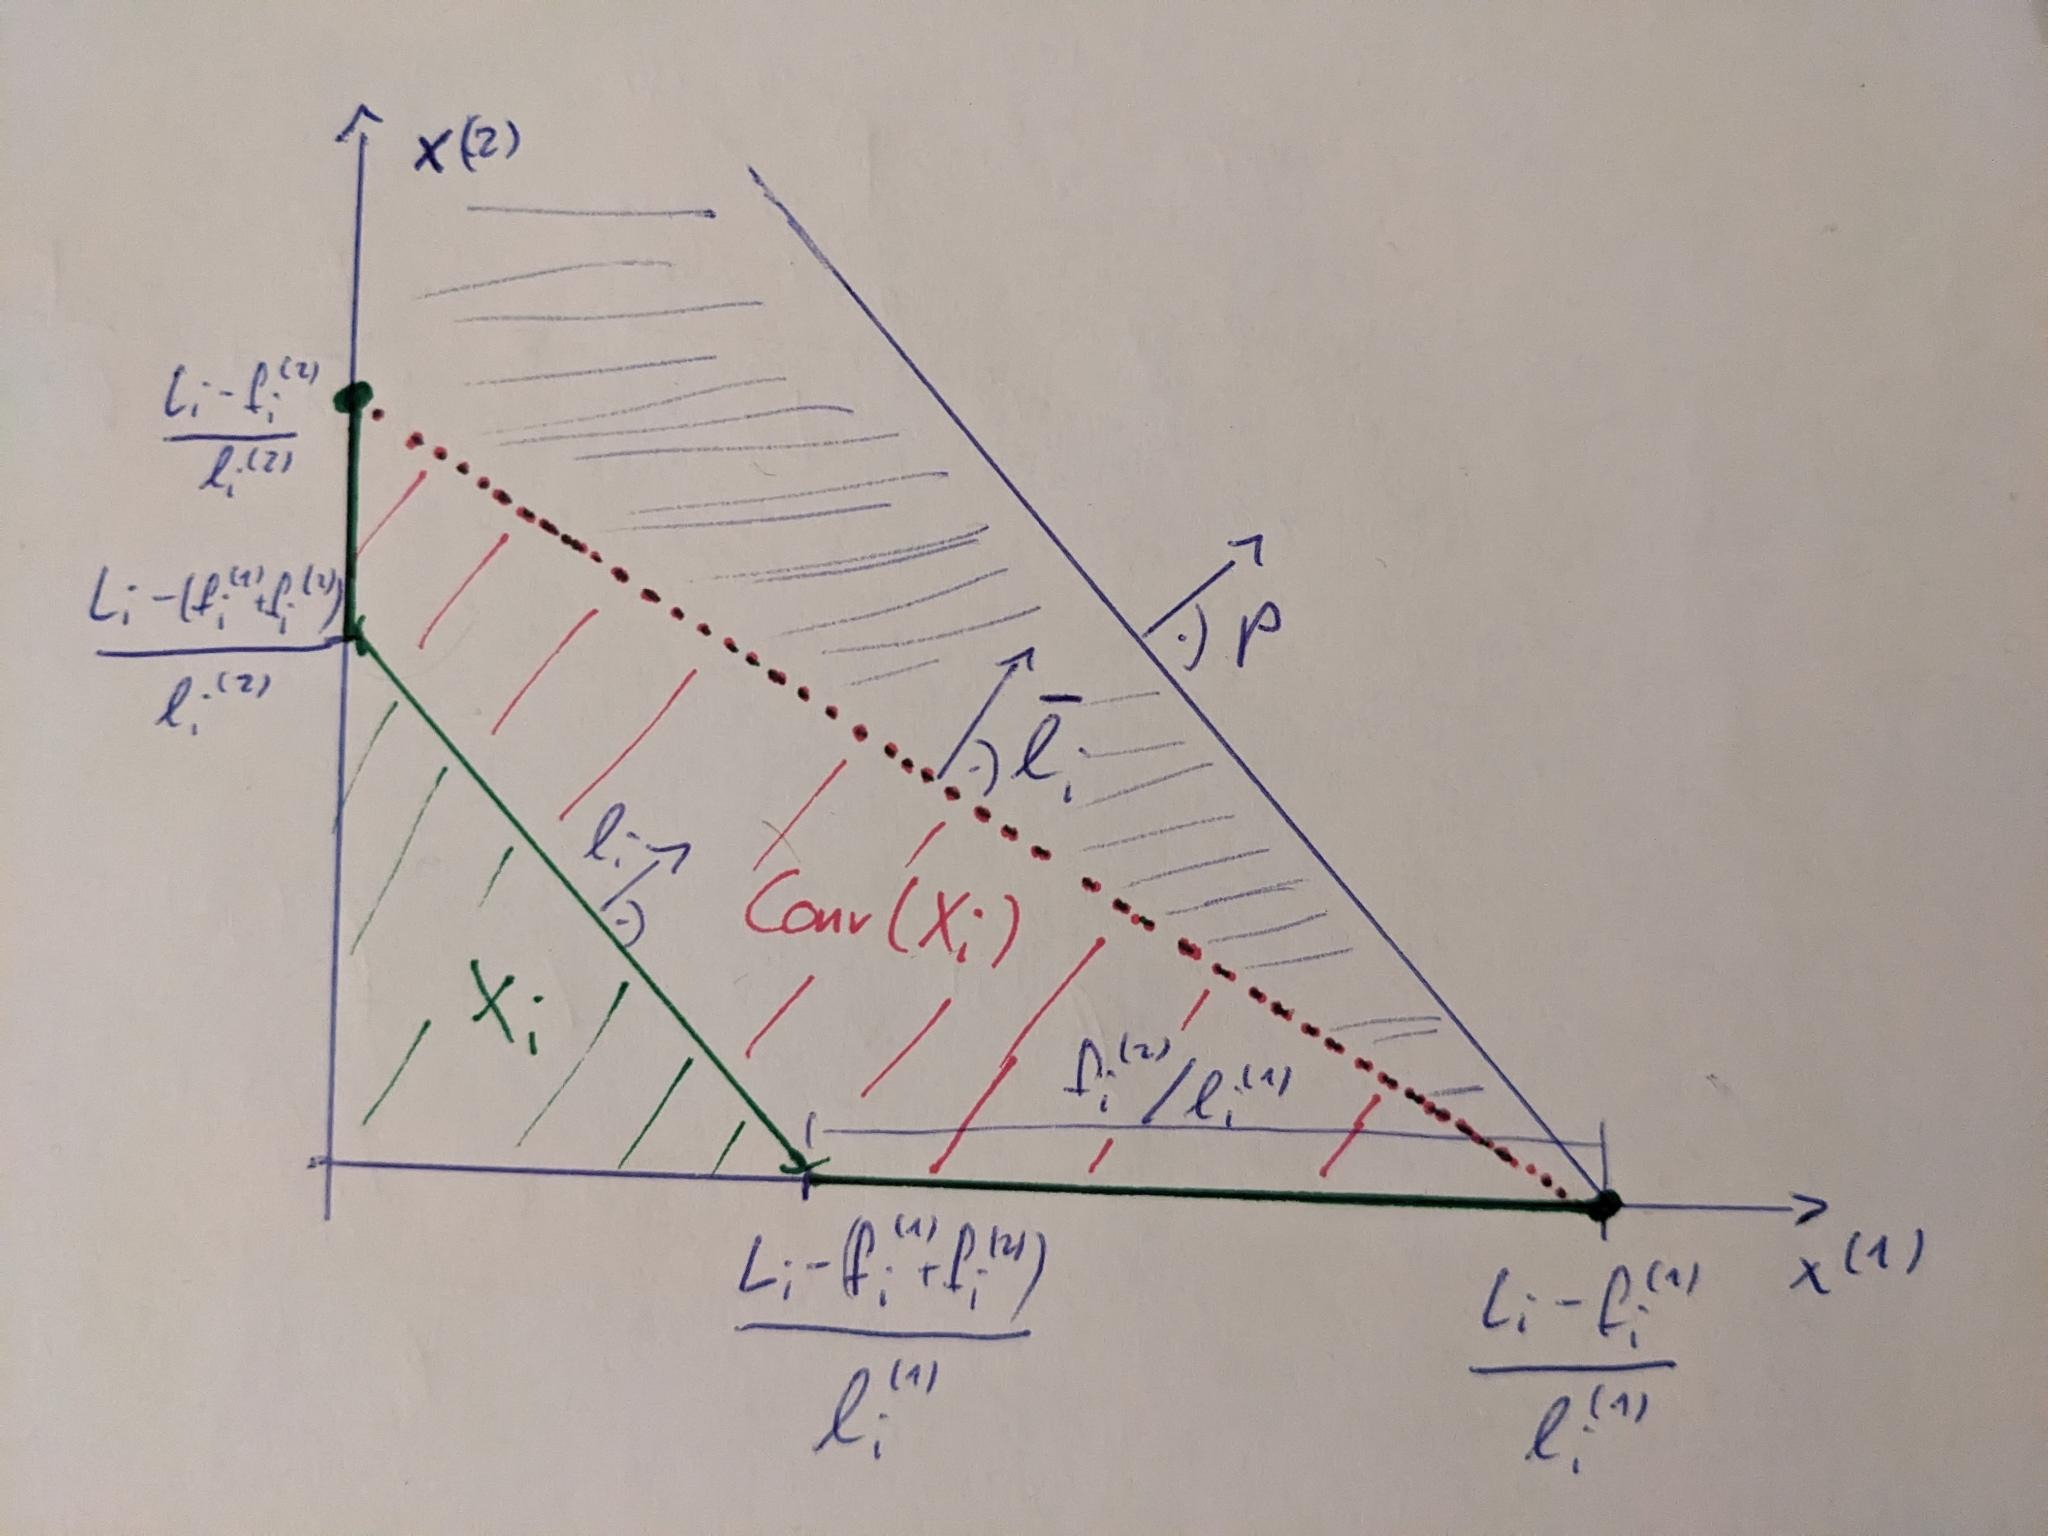
\includegraphics[width=0.95\textwidth]{images/conv_hull_vs_trade.jpeg}
	\centering
	\caption{
		The convex hull \(\conv(X_i)\) is larger than \(X_i\). But trade might
		be an improvement even still. Trade is always at least as good as the
		convex hull. The more different \(p\) from \(\bar{l}_i\) the better for
		individual \(i\). If \(p\) and \(\bar{l}_i\) were equal only
		\(\conv(X_i)\) would be available for consumption.
	}
\end{figure}

\begin{figure}
	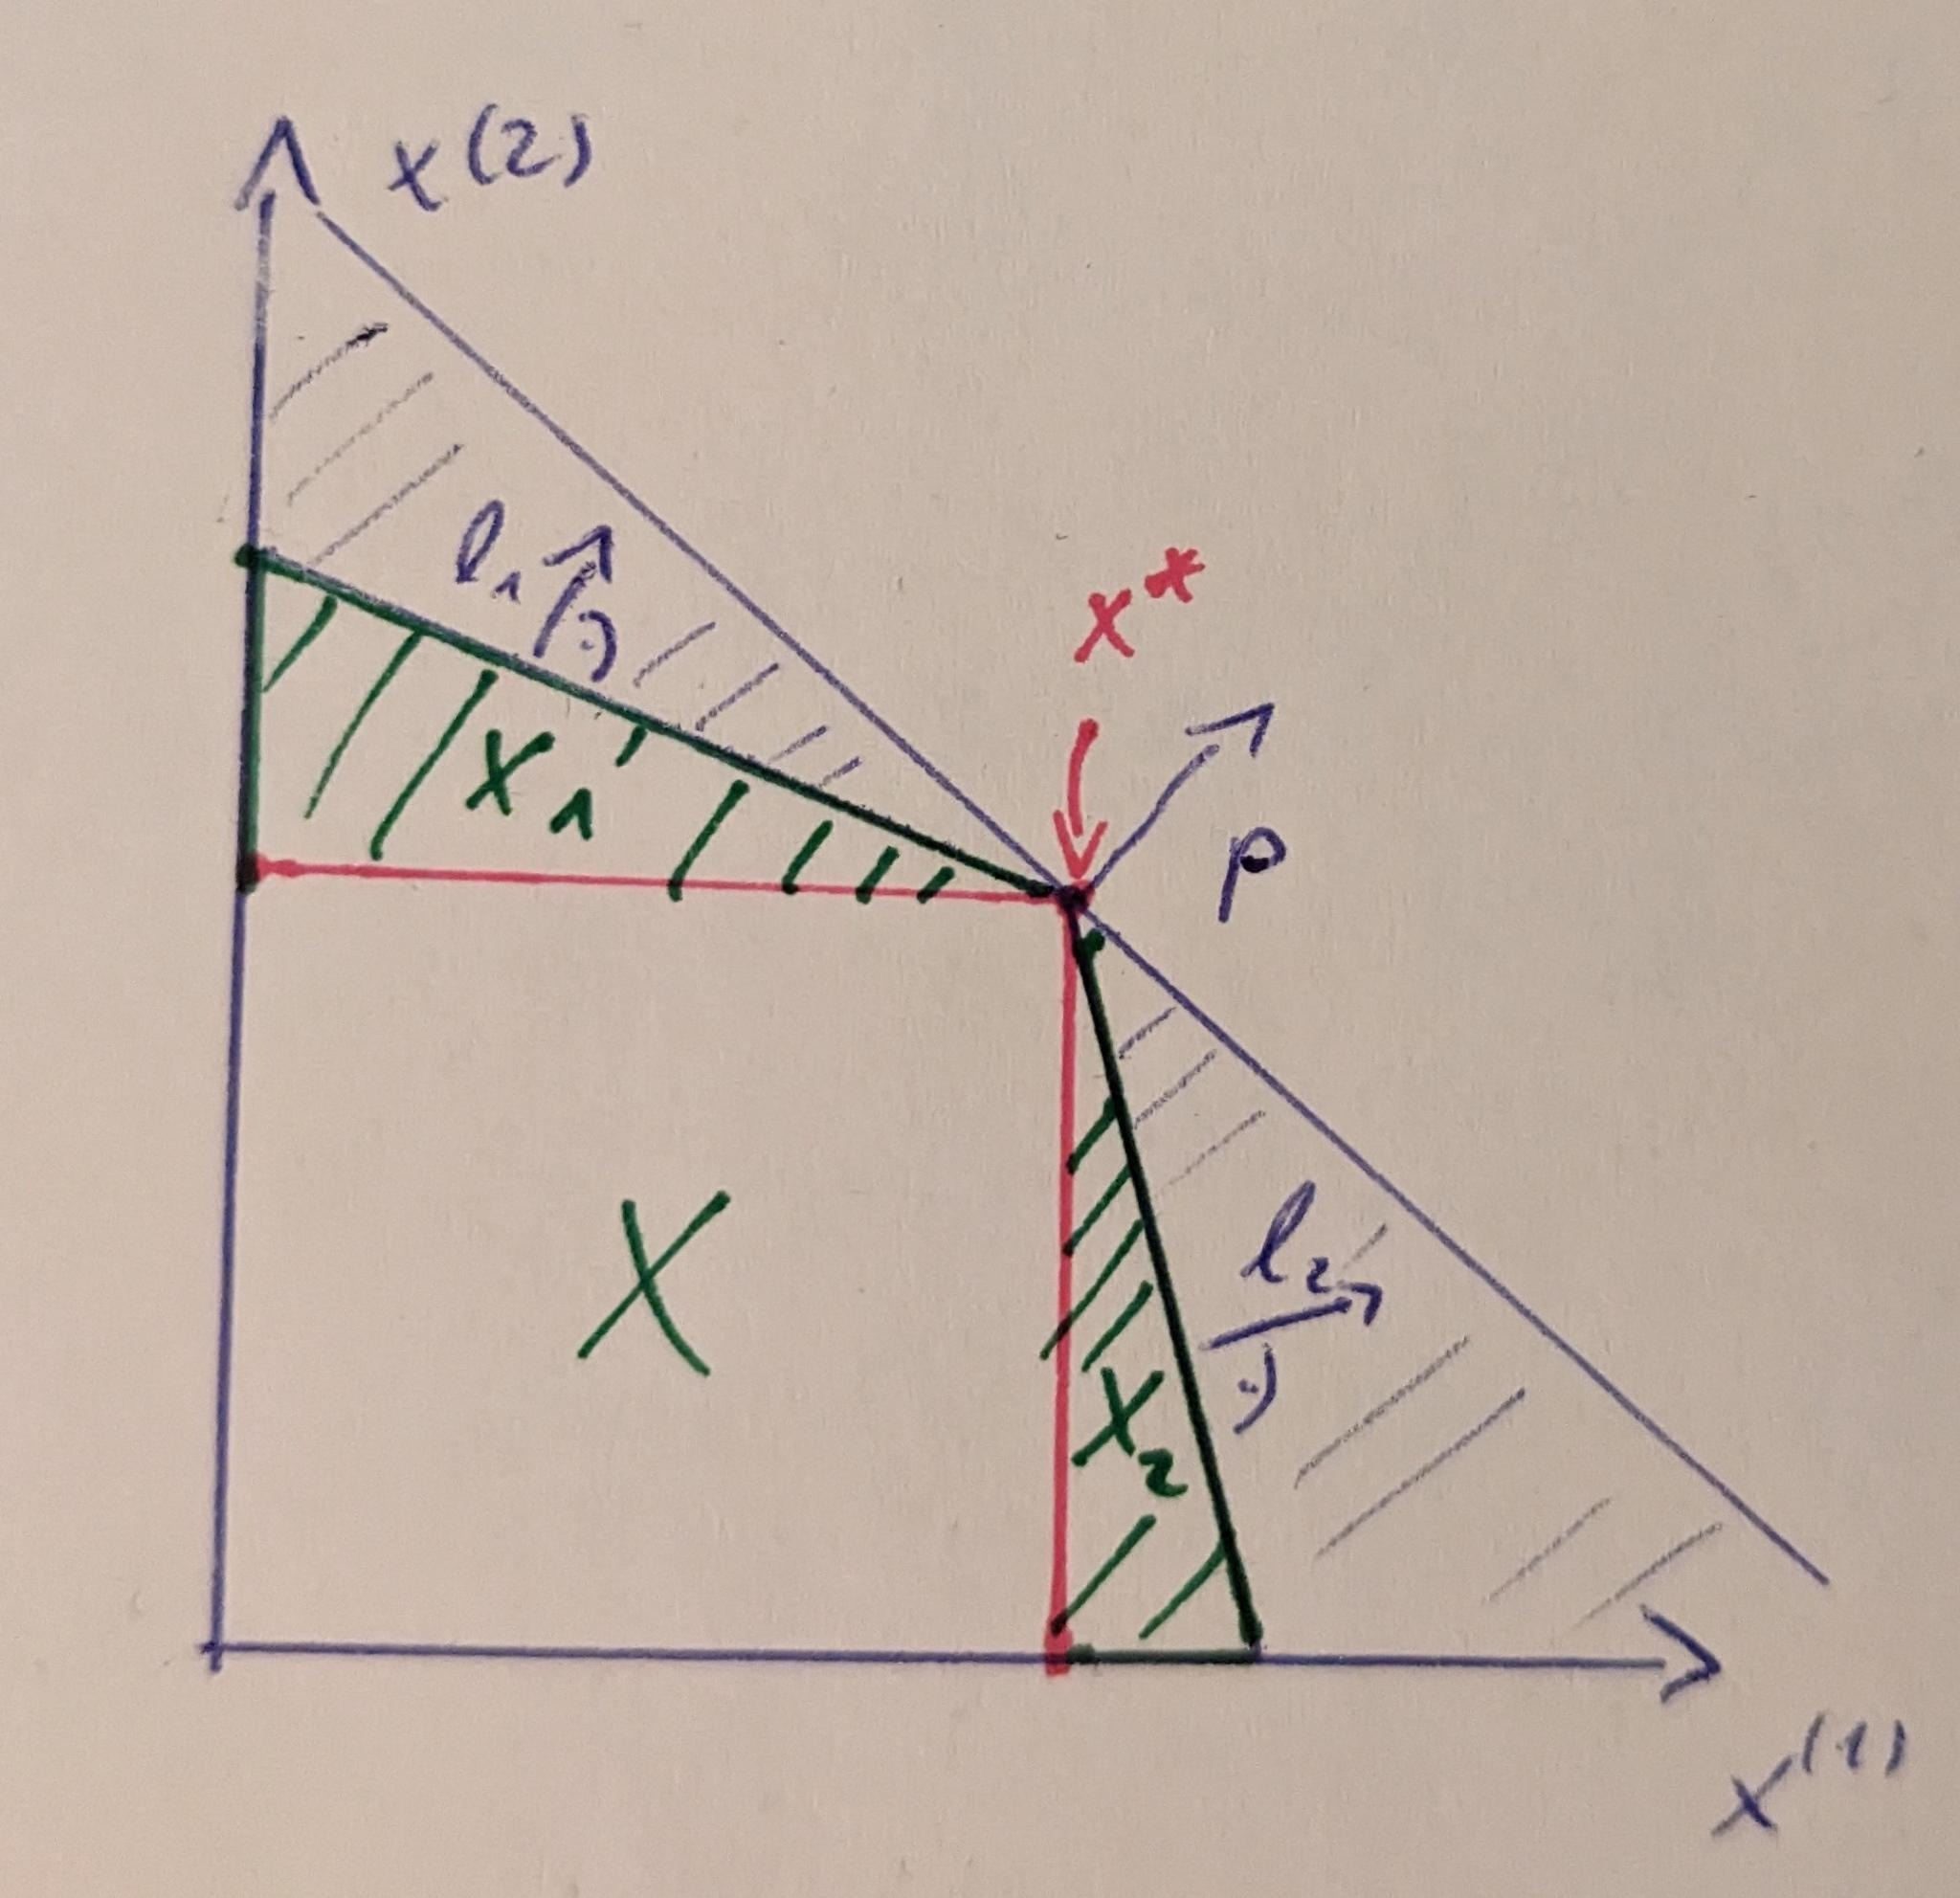
\includegraphics[width=0.3\textwidth]{images/2_people_trade_fair.jpeg}
	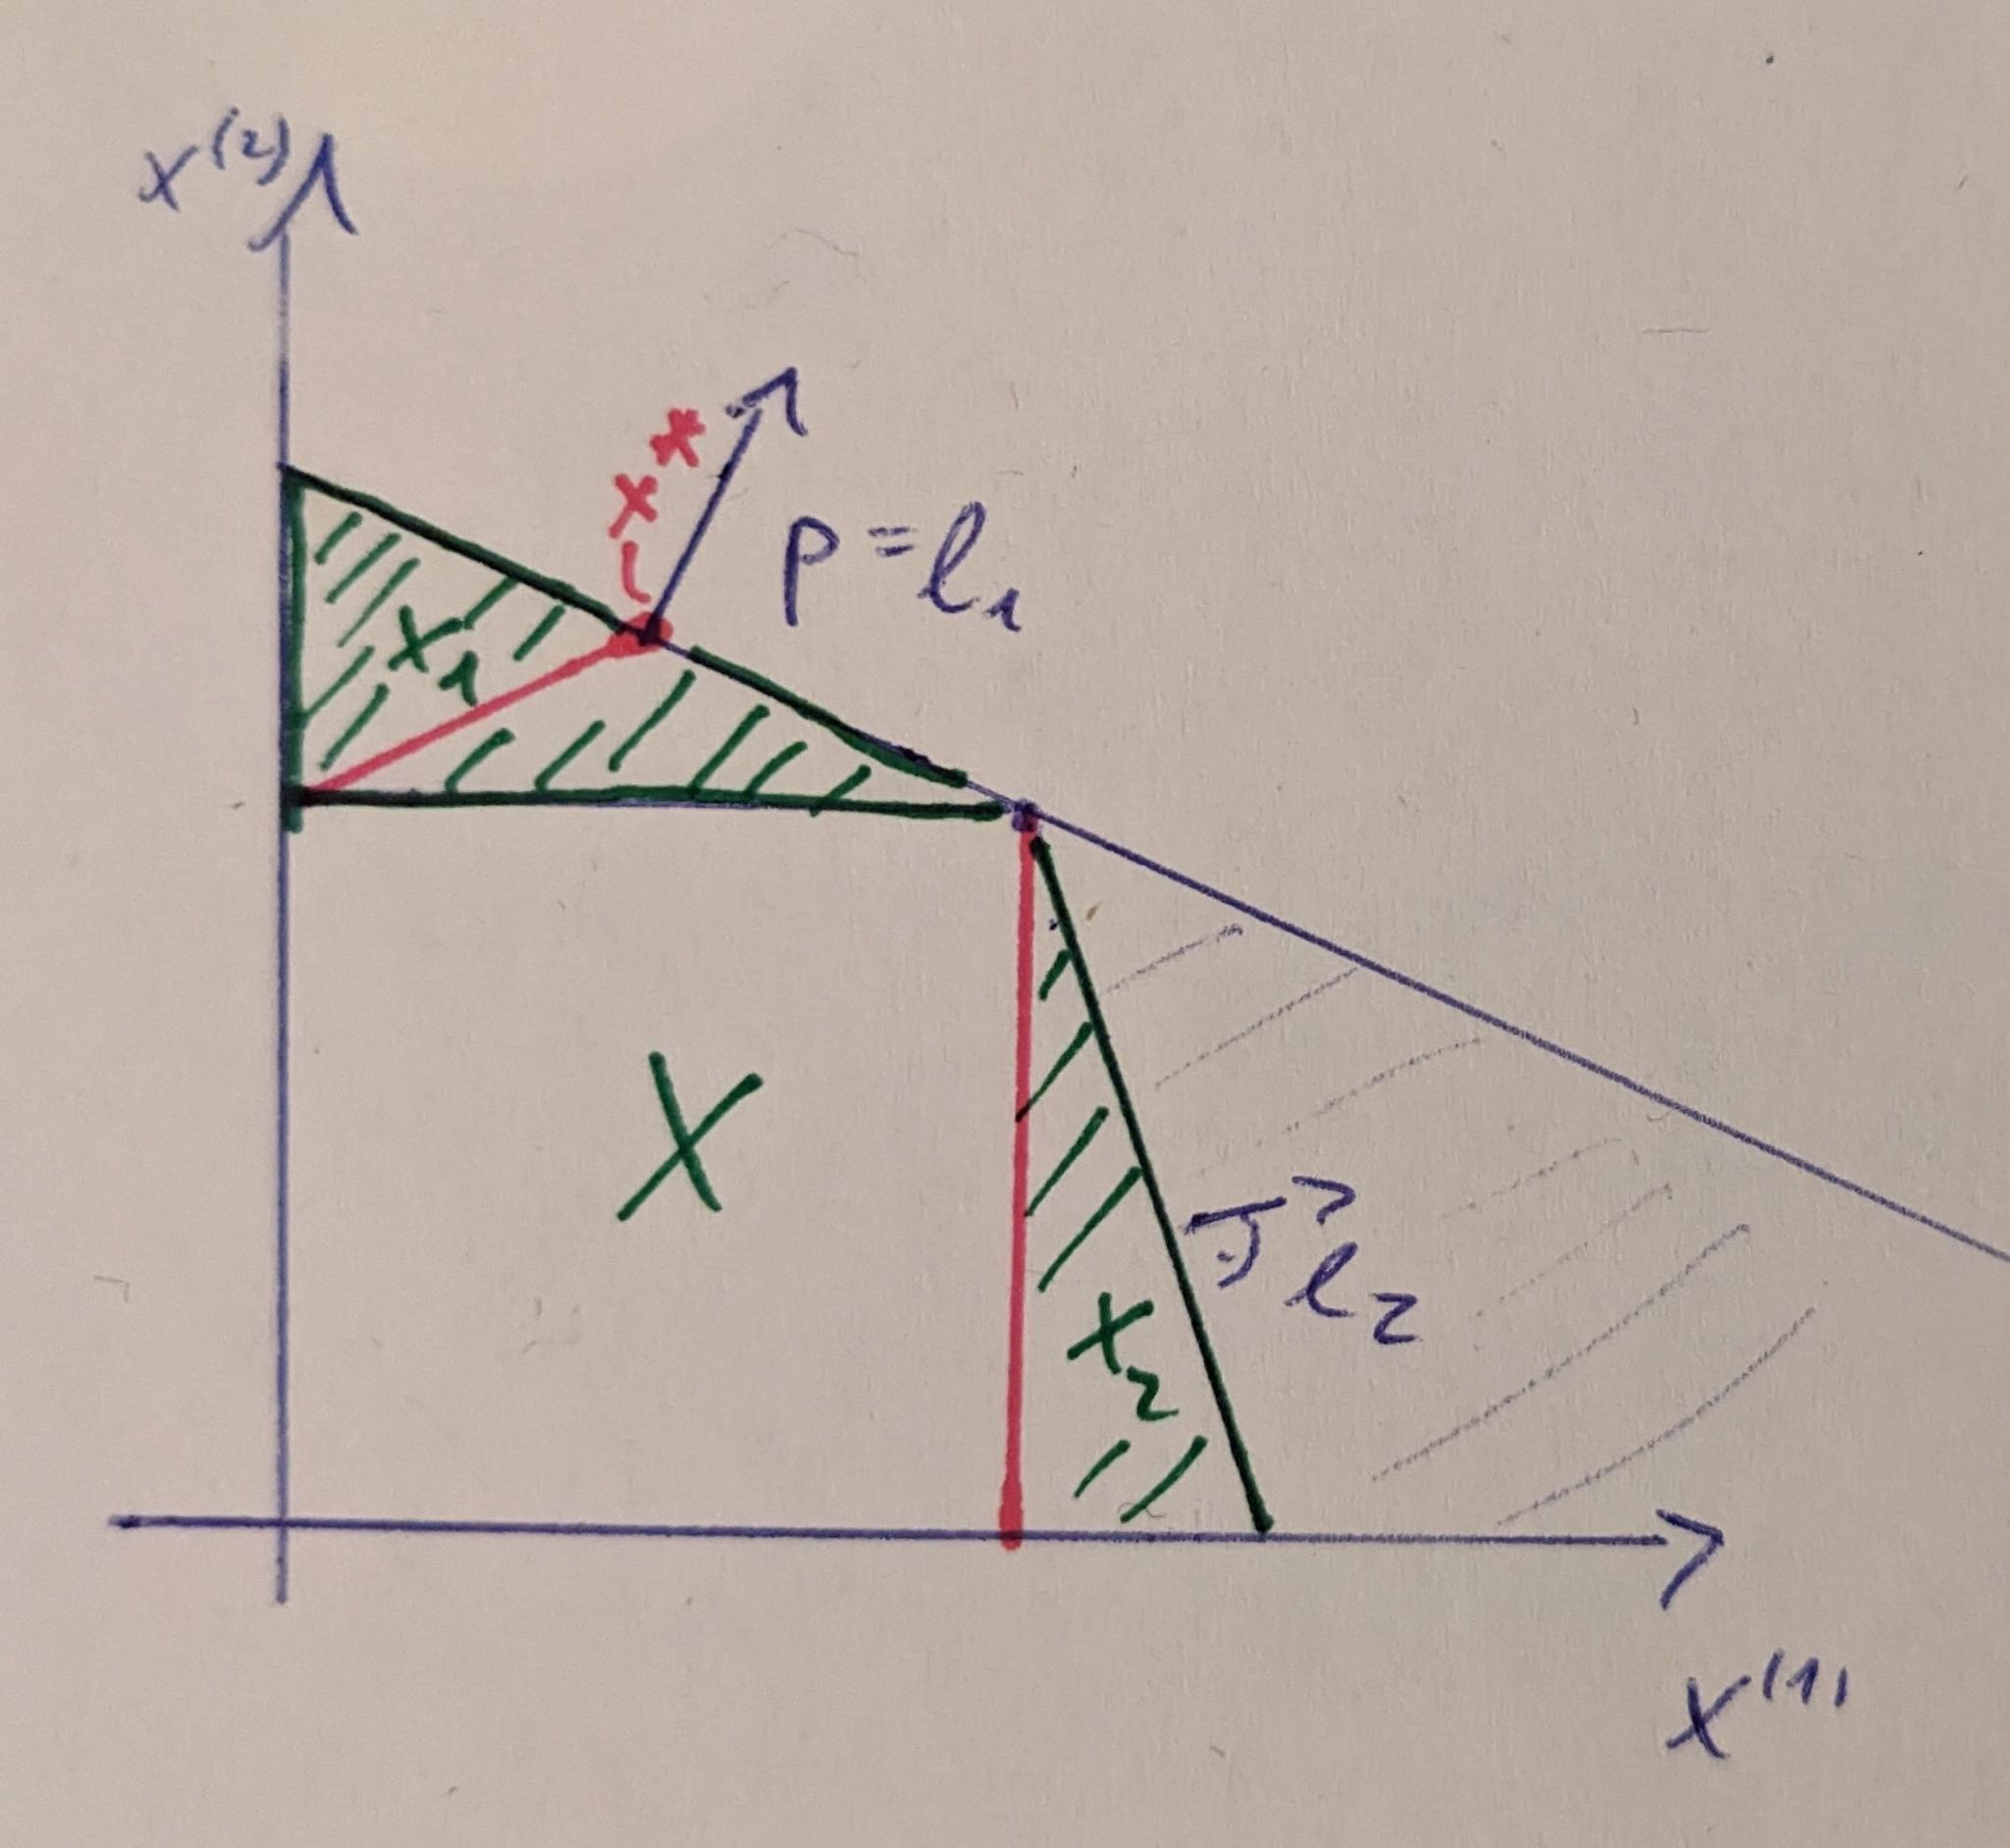
\includegraphics[width=0.315\textwidth]{images/2_people_trade_half_specialization.jpeg}
	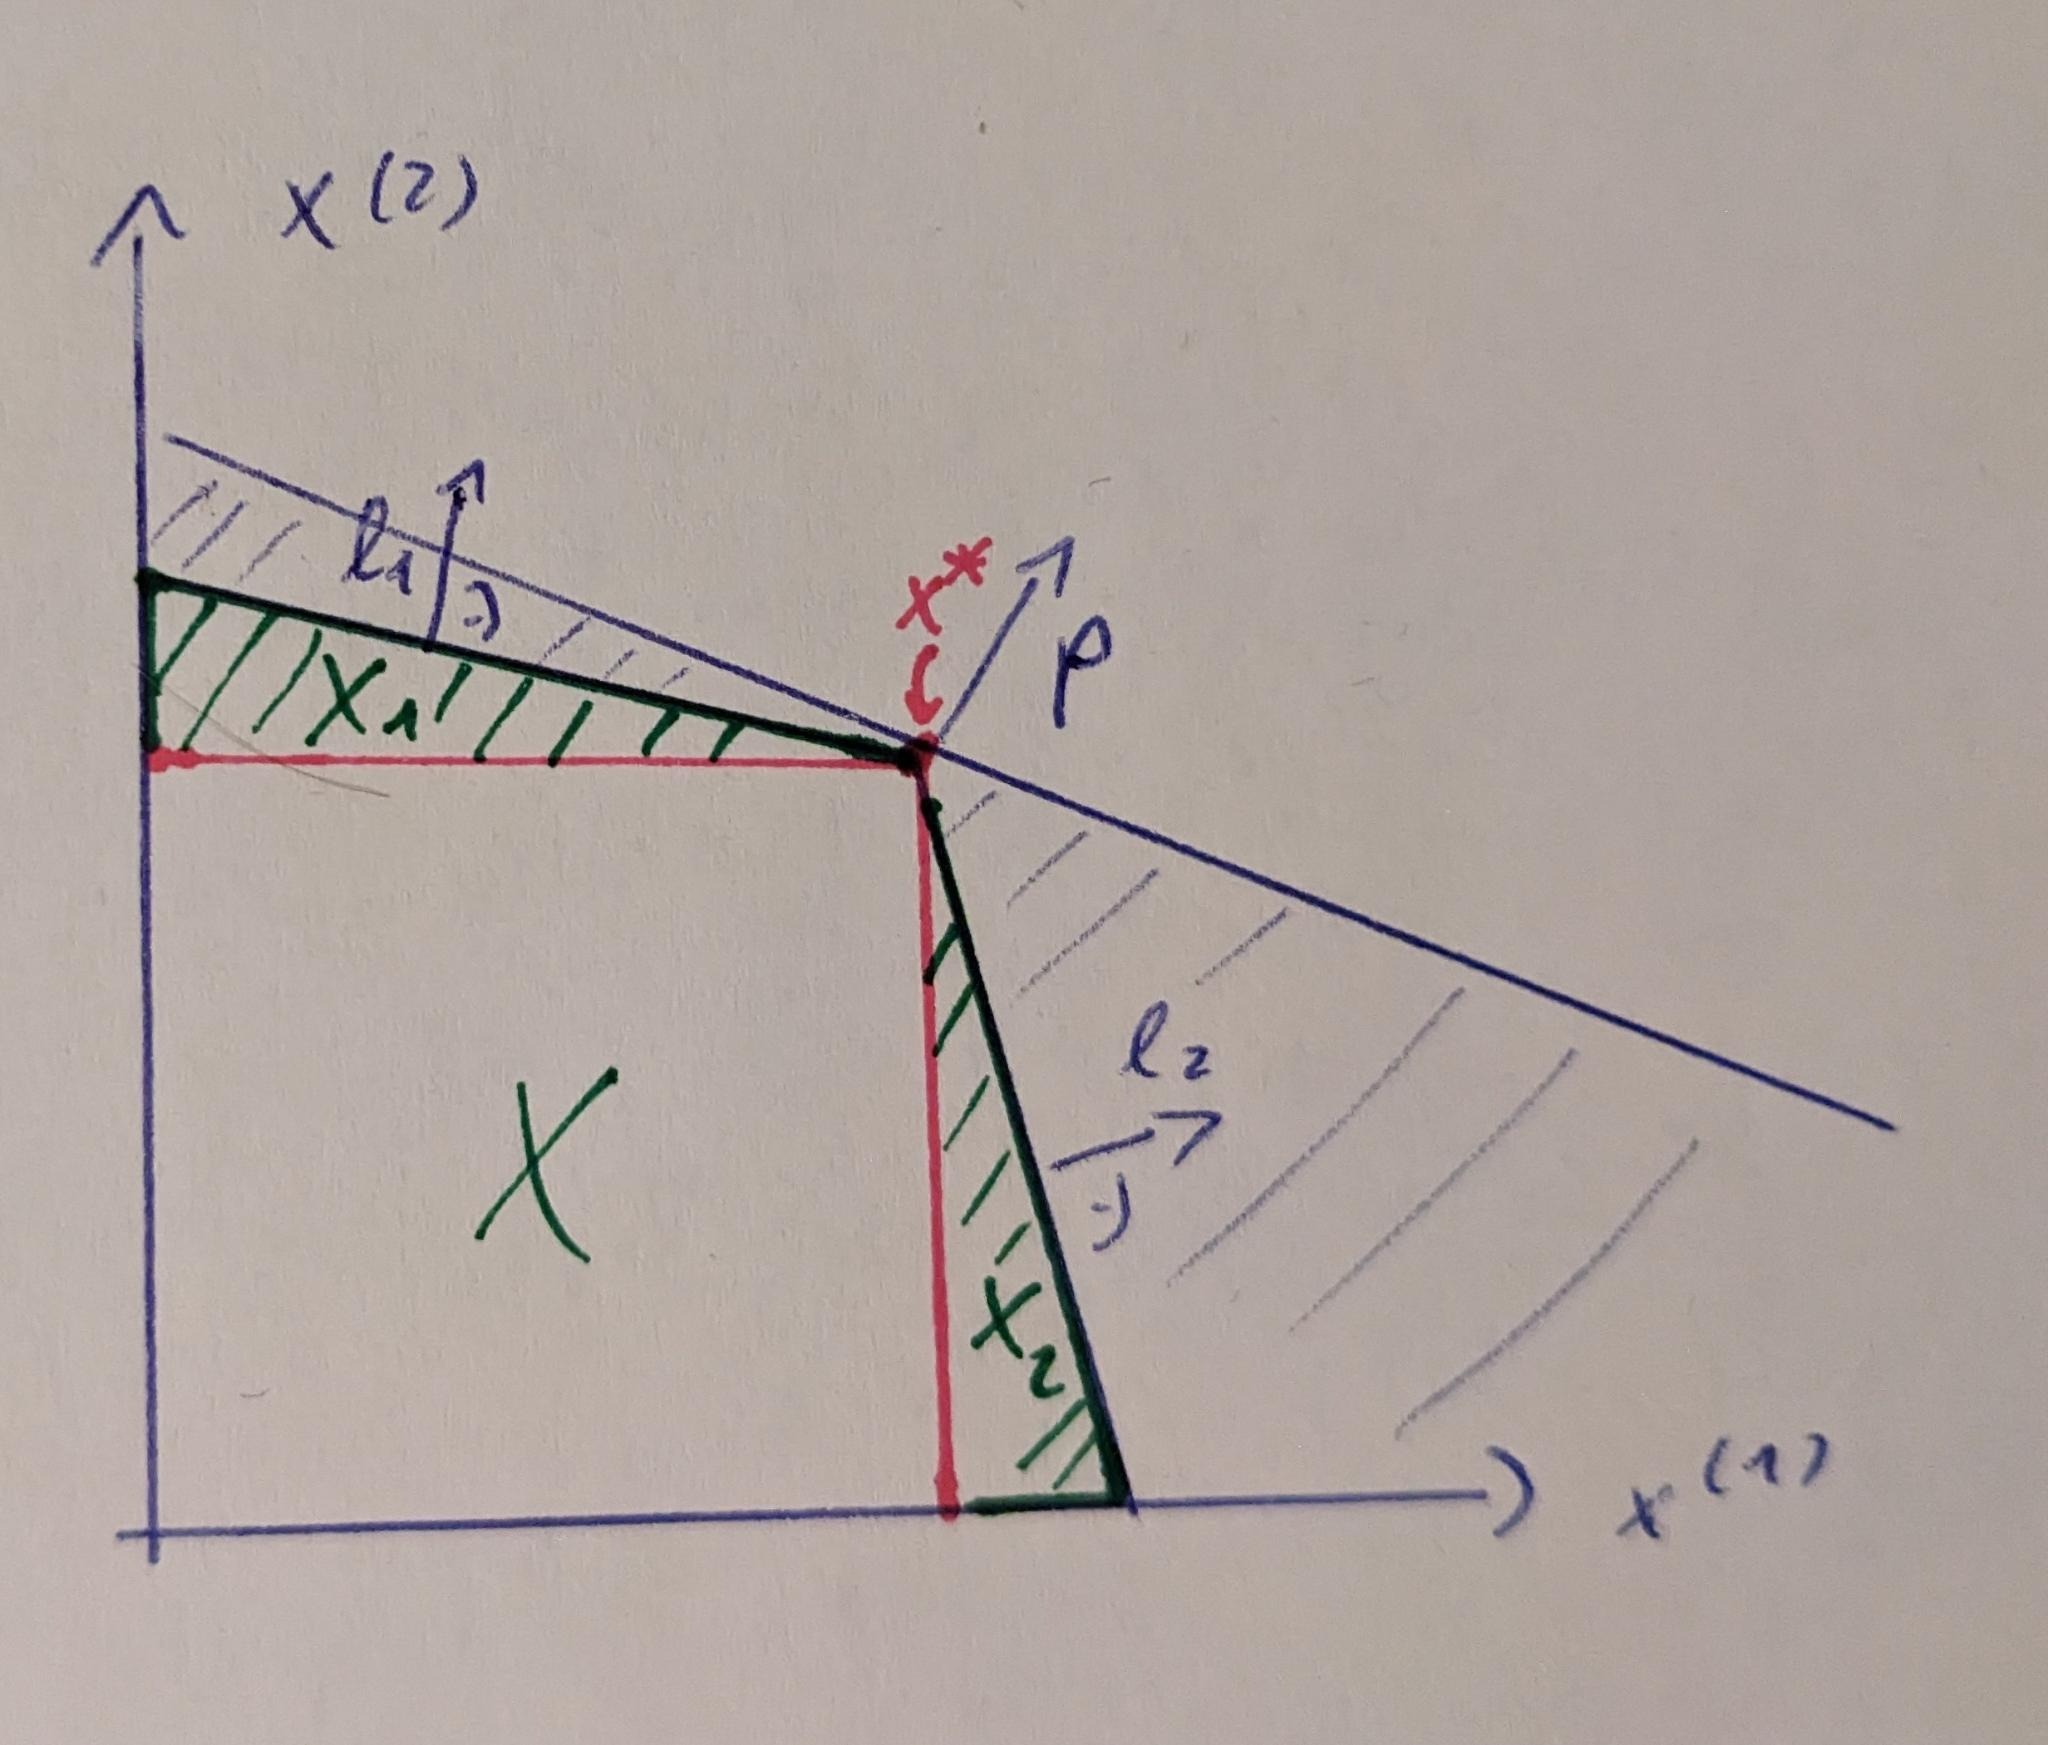
\includegraphics[width=0.34\textwidth]{images/2_people_trade_unfair.jpeg}
	\caption{
		Two people with different skills producing \(x^*\) together. In the first
		picture person \(i\) specializes on producing \(i\) and they both gain
		from this trade as \(p\) is different from \(l_i\). In the second picture,
		person \(1\) produces both goods. The price vector has to be a multiple of
		\(l_1\), otherwise person \(1\) would focus on one of the two goods.
		Person \(1\) does not gain anything from trade. In the third picture, both
		are specialized and both gain from trade, but the gains of person \(2\)
		are larger than person \(1\) as \(p\) is closer to \(l_1\) in direction.
	}
\end{figure}

\begin{figure}
	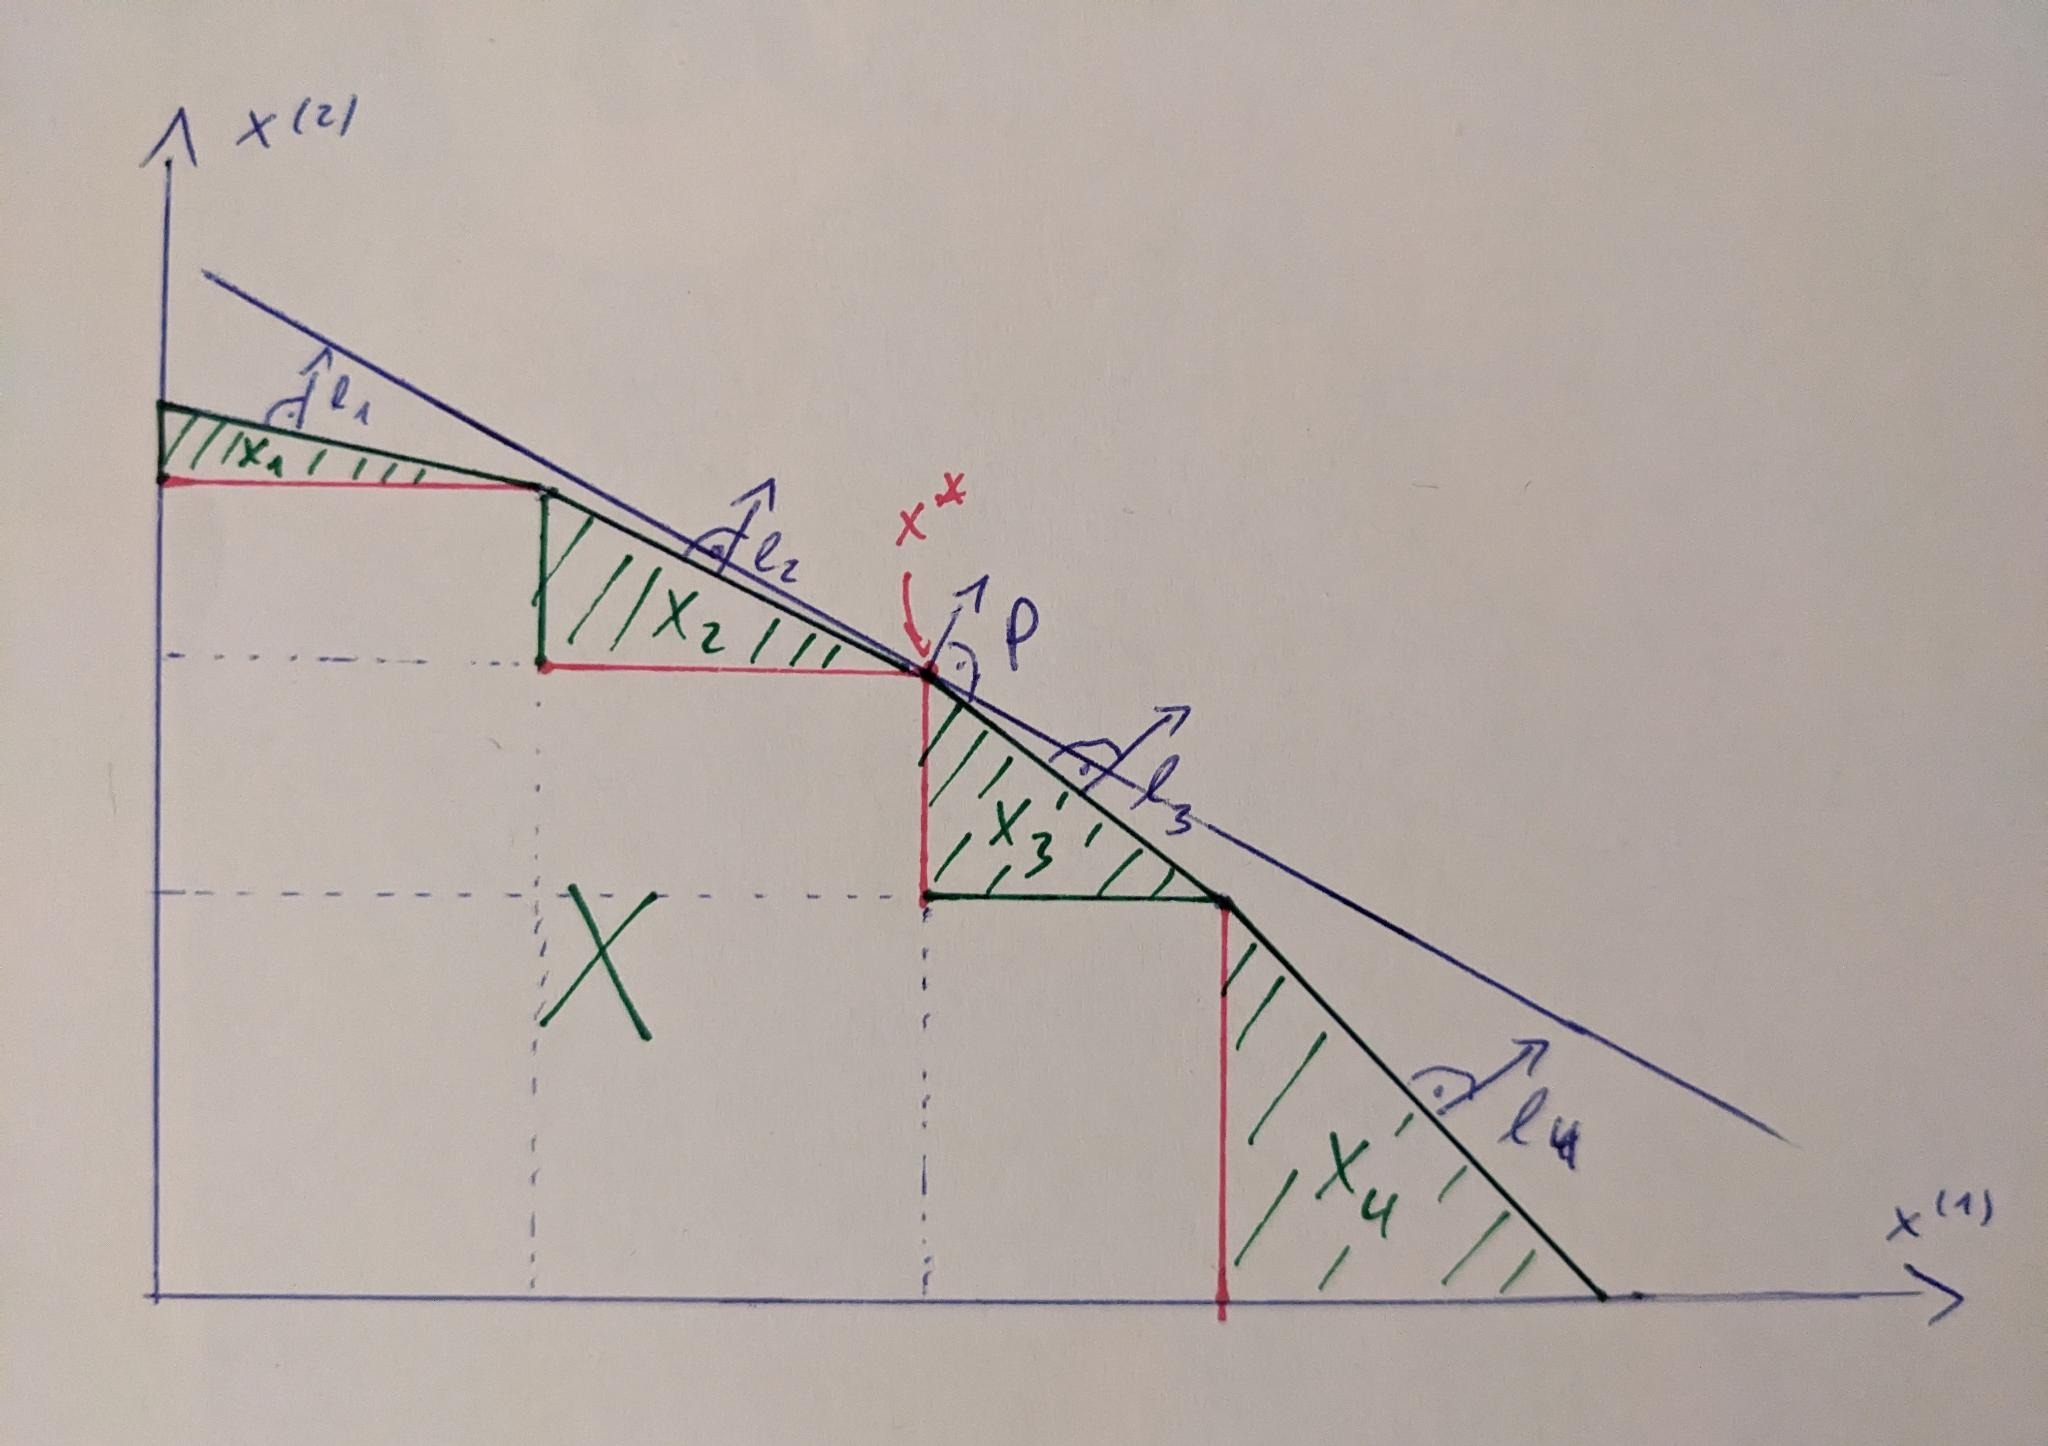
\includegraphics[width=0.95\textwidth]{images/4_people_trade.jpeg}
	\caption{
		Four people are producing \(x^*\) together. The more specialized people
		on the edges \(1,4\) gain more from this trade than the people in the
		middle, where \(p\) is more similar to \(l_i\). The more people you add
		the, smoother the border of \(\bar{X}_n\) should become. The edges
		give us the opportunity to pick \(p\) in a range of the adjacent \(l_i\).
		A smooth border would give us no choice, as \(p\) would have to be
		tangential. Also notice that fixed costs for individuals matter less and
		less with more people, as almost nobody needs to produce more than one
		good. For this essentially remove the upper right part of the triangles
		of the \(X_i\) and observe that the points on the outer surface would
		still move together and become a continuous curve for large numbers of
		people.
	}	
\end{figure}

You should get the intuition that we can achieve any \(x^*\) in the ``production
frontier'' of \(X\) with positive prices (this is the topic of Section~\ref{sec:
production frontier}). And that this price is essentially fully determined if
enough people participate as supply becomes a continuous function (which will be
the topic of Section~\ref{sec: shape supply/demand}). Lastly you
should understand how people would like prices to be dissimilar to their own
skills. Highly specialized people gain more from trade than generalists.

\FloatBarrier
